% XCircuit output "ckt_2.tex" for LaTeX input from ckt_2.eps
\def\putbox#1#2#3#4{\makebox[0in][l]{\makebox[#1][l]{}\raisebox{\baselineskip}[0in][0in]{\raisebox{#2}[0in][0in]{\scalebox{#3}{#4}}}}}
\def\rightbox#1{\makebox[0in][r]{#1}}
\def\centbox#1{\makebox[0in]{#1}}
\def\topbox#1{\raisebox{-0.60\baselineskip}[0in][0in]{#1}}
\def\midbox#1{\raisebox{-0.20\baselineskip}[0in][0in]{#1}}
   \scalebox{0.76494}{
   \normalsize
   \parbox{2.61458in}{
   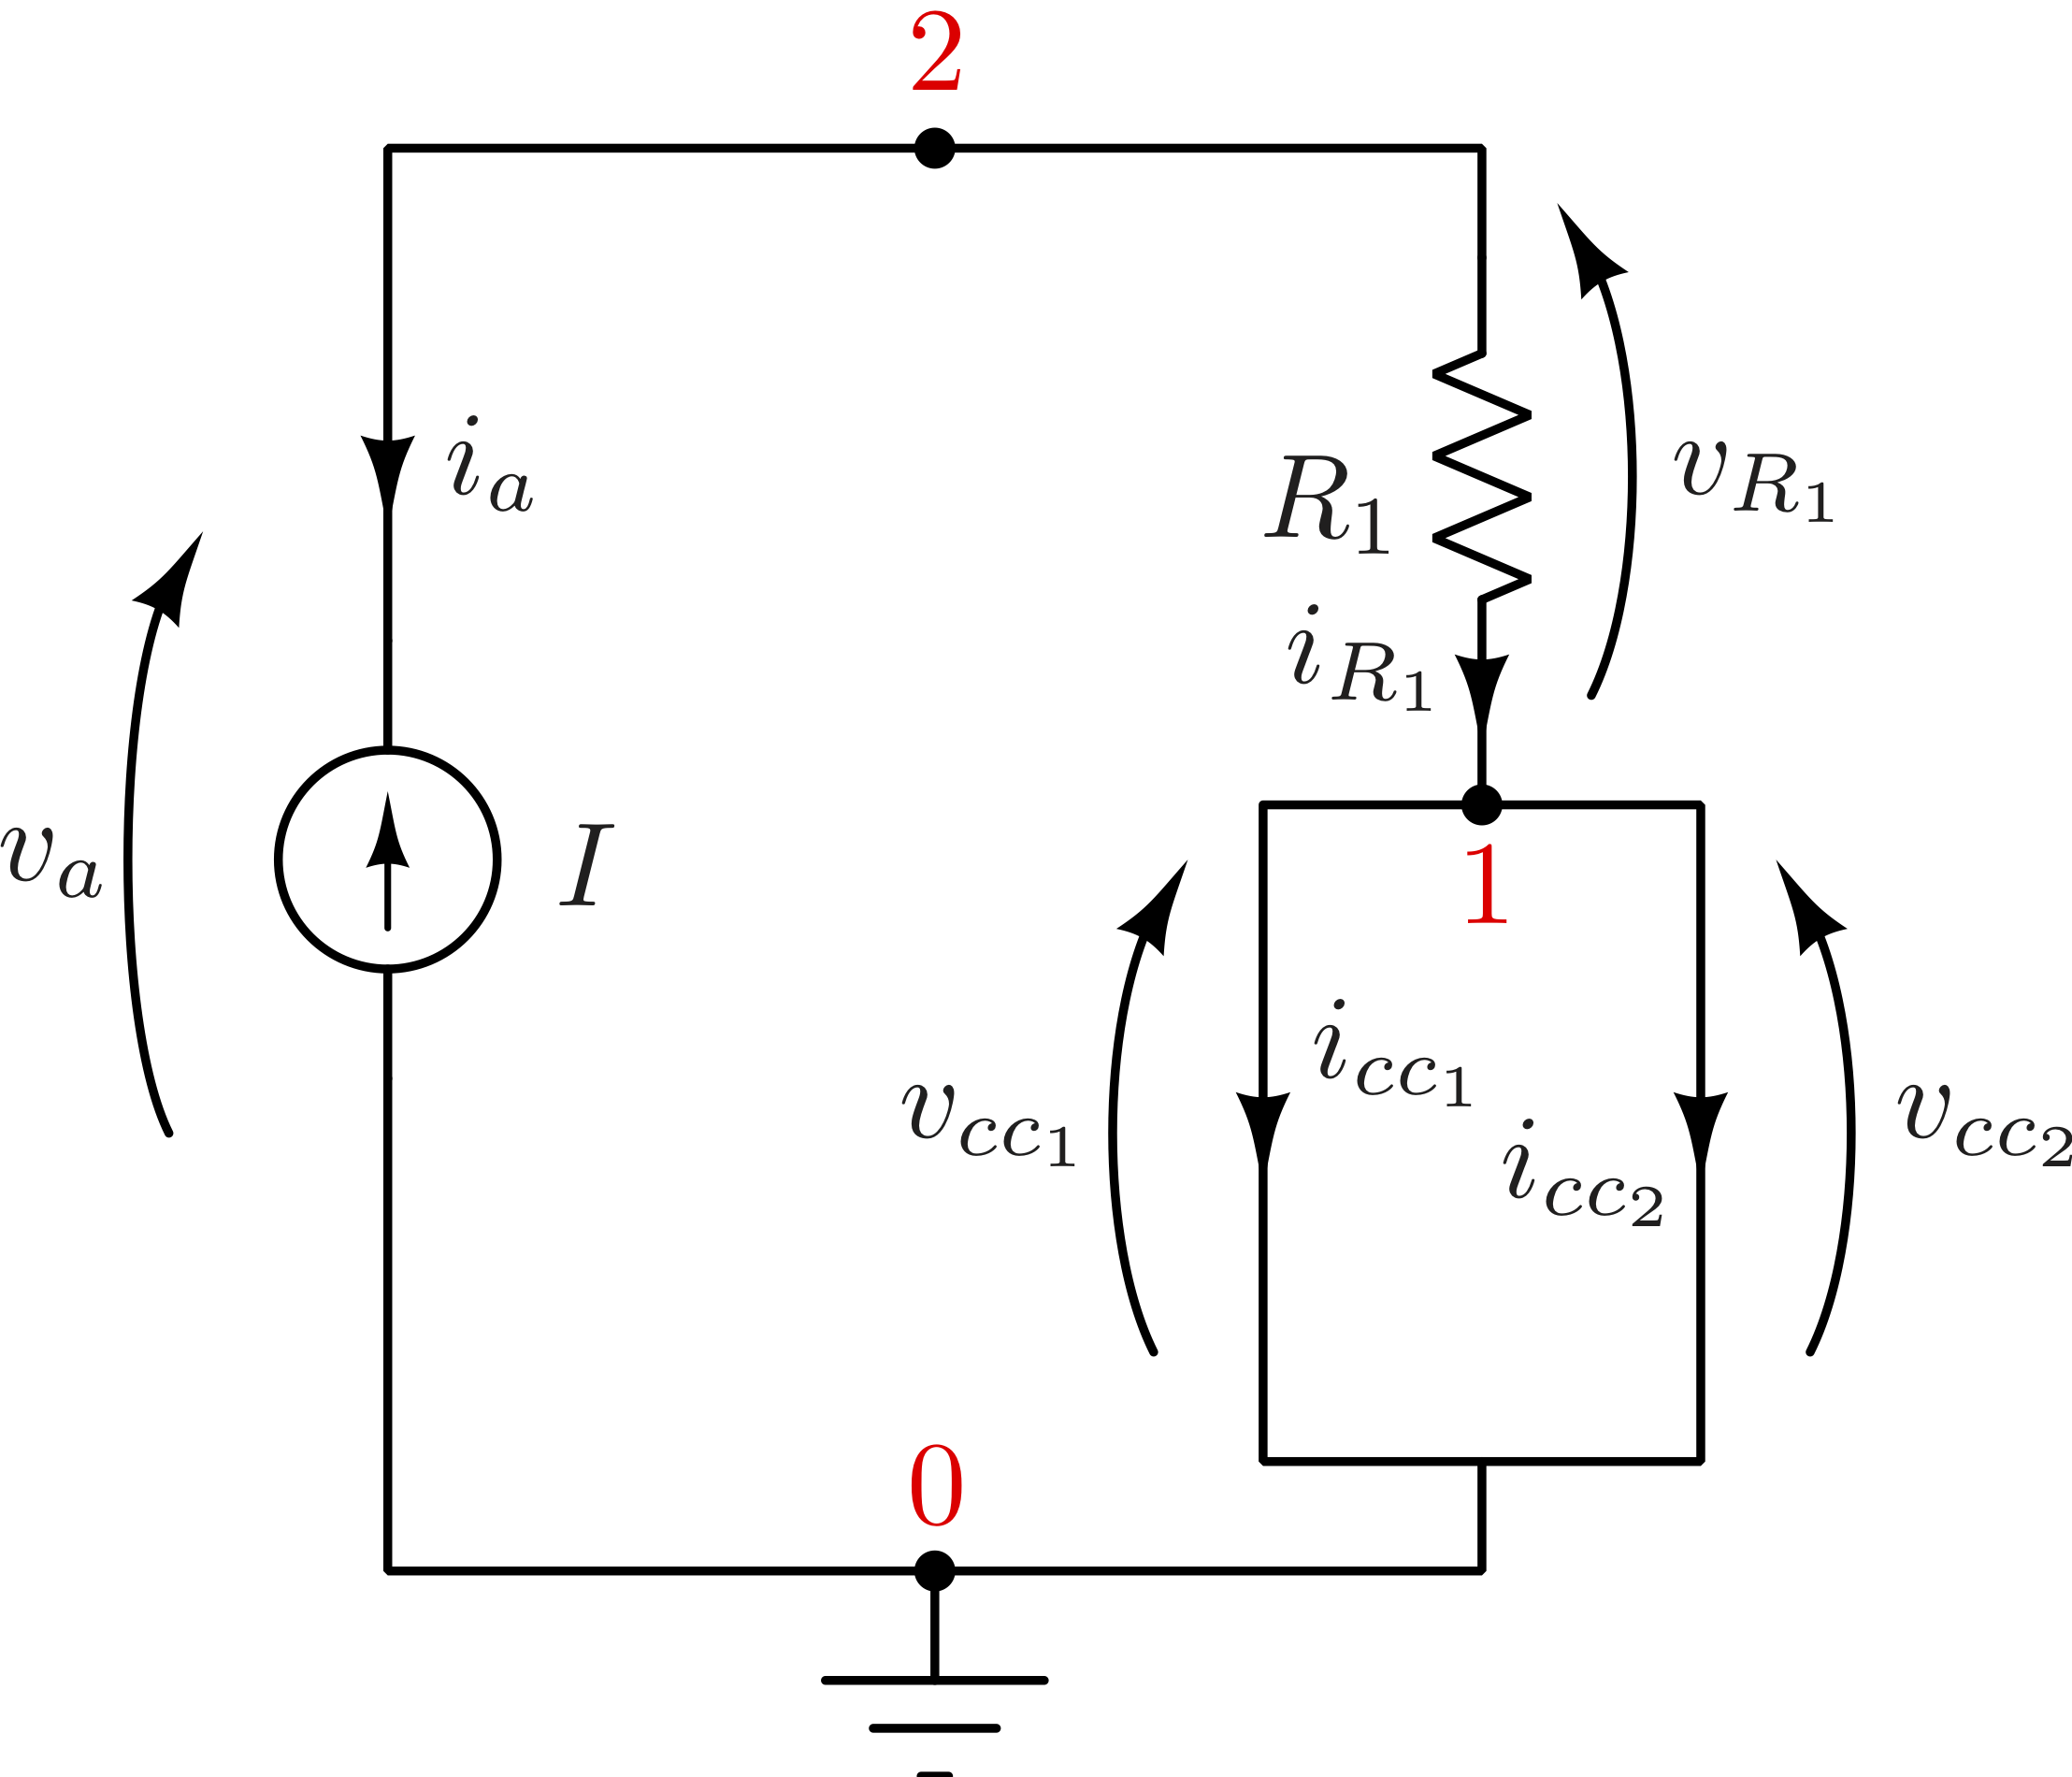
\includegraphics[scale=1]{ckt_2}\\
   % translate x=710 y=503 scale 0.29
   \putbox{0.96in}{0.35in}{1}{\textcolor{red}{0}}%
   \putbox{1.6in}{1.05in}{1}{\textcolor{red}{1}}%
   \putbox{0.96in}{2.02in}{1}{\textcolor{red}{2}}%
   \putbox{0.55in}{1.07in}{1}{$I$}%
   \putbox{1.37in}{1.5in}{1}{$R_1$}%
   \putbox{-0.1in}{1.1in}{1}{$v_a$}%
   \putbox{0.42in}{1.55in}{1}{$i_a$}%
   \putbox{1.85in}{1.55in}{1}{$v_{R_1}$}%
   \putbox{1.4in}{1.33in}{1}{$i_{R_1}$}%
   \putbox{0.95in}{0.80in}{1}{$v_{cc_1}$}%
   \putbox{1.43in}{0.87in}{1}{$i_{cc_1}$}%
   \putbox{2.11in}{0.80in}{1}{$v_{cc_2}$}%
   \putbox{1.65in}{0.73in}{1}{$i_{cc_2}$}%
   } % close 'parbox'
   } % close 'scalebox'
   \vspace{-\baselineskip} % this is not necessary, but looks better
